\documentclass{standalone}
\usepackage{tikz}
\usepackage{graphicx}
\usetikzlibrary{shapes.geometric, backgrounds}

\begin{document}
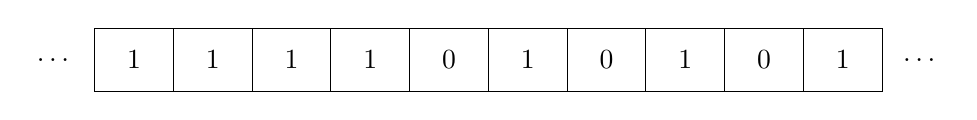
\begin{tikzpicture}

    % Línea de celdas con valores más cerca de las imágenes de los autos
    \foreach \x/\val in {-2/1, -1/1, 0/1, 1/1, 2/0, 3/1, 4/0, 5/1, 6/0, 7/1} {
        \draw (\x,-1) rectangle ++(1,-0.8);
        \node at (\x+0.5,-1.4) {\val};
    }
    
    % Puntos suspensivos (quitando las celdas de los extremos)
    \node at (-2.5,-1.4) {\ldots};
    \node at (8.5,-1.4) {\ldots};
\end{tikzpicture}
\end{document}
